\chapter{Radioactive Decay}
\section{Radioactivity}
Many nuclides present in the universe are unstable and spondaneously change in to other nuclides by a process pulled radioactive decay. The phenomina is known as radioactivity and was discovered Antonine Bequerel. Following three aspects of radioactivity are extraordinary from the perspective of classical physics.\\
(i) \quad When a nucleus undergo $\alpha$ or $\beta$ decays its atomic number $Z$ changes and it becomes the nucleus of a different form. Obviously the elements are not immutable. (not transformed to the original one naturally)\\
(ii)\quad The energy liberated during radioactive decay comes from with in the individual nuclei without external excitation.\\
(iii)\quad Radioactive decay is statistical process.
\subsection{Radioactive Decay}
There are five different ways in which a radio action nuclide can decay . That are by emitting an alpha ($ ^4_2He$ nuclei), beta(electrons),gamma(high energy photons) particles or by positron emission  and electron capture. In which alpha particle is +vely charged and $P$ particles are -vely charged and the gamma rays are natural. The penitrating power is maximum for  gamma rays. The penitrating power of $\alpha$,$\beta$,$\gamma$, particle can be picturized as\\
\begin{figure}[H]
	\centering
	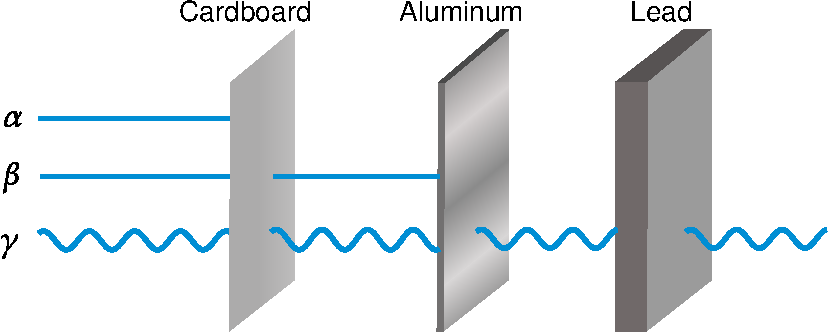
\includegraphics[height=3cm,width=8cm]{diagram-20220307(6)-crop}
	\caption{}
	\label{}
\end{figure}
Radioactive Decay\\
	\begin{table}[H]
	\centering
	\renewcommand*{\arraystretch}{1.5}
	\begin{tabular}{|p{2.5cm} |p{3.5cm}|p{4cm}|p{3.7cm} |}
	\hline Decay &Reason for instability& Transformation & Example \\
	\hline Alpha decay &Nucleus is too large.& ${ }_{2}^{A} X \rightarrow{ }_{Z-2}^{A-4} Y+{ }_{2}^{4} \mathrm{He}$ & ${ }_{29}^{238} \mathrm{U} \rightarrow{ }_{90}^{234} \mathrm{Th}+{ }_{2}^{4} \mathrm{He}$ \\
	 & &Emission of $\alpha$-particle reduces size of nucleus.& \\
	\hline
	Beta decay &Nucleus has too many neutrons relative to number of protons.& ${ }_{2}^{A} X \rightarrow{ }_{Z+1}^{A} Y+e^{-}$ & ${ }_{6}^{14} \mathrm{C} \rightarrow{ }_{7}^{14} \mathrm{~N}+e^{-}$ \\
	 & &Emission of electron by neutron in nucleus changes the neutron to a proton.& \\
		\hline
	Gamma decay &Nucleus has excess energy.& ${ }_{Z}^{A} X^{*} \rightarrow{ }_{Z}^{A} X+\gamma$ & ${ }_{87}^{87} \mathrm{Cu}+{ }_{38}^{8} \mathrm{Sr}^{*} \rightarrow{ }_{38}^{87} \mathrm{Sr}+\gamma$ \\
	 & &Emission of $\gamma$-ray reduces energy of the nucleus.& \\
		\hline
	Electron capture &Nucleus has too many protons relative to number of neutrons.& ${ }_{Z}^{A} X+e^{-} \rightarrow_{z-1}^{A} Y$ & ${ }_{64}^{A} \mathrm{Cu}+e^{-} \rightarrow{ }_{28}^{64} \mathrm{Ni}$ \\
	 & &Capture of electron by protons changes the proton to a neutron.& \\
		\hline
	Positron emission &Nucleus has too many protons relative to number of neutrons.& ${ }_{2}^{A} X \rightarrow{ }_{-1}^{A} Y+e^{+}$ & ${ }_{29}^{64} \mathrm{Cu} \rightarrow{ }_{28}^{64} \mathrm{Ni}+e^{+}$ \\
	 & &Emission of positron by proton in nucleus changes the proton to a neutron.& \\
	\hline
	\end{tabular}
\end{table}





${ }^{+}$The * denotes an excited nuclear state and $\gamma$ denotes a gamma-ray photon.
\subsection{Activity}
The activity of a sample of any radioactive nuclide is the rate at which the nuclei of its constituent atoms decay.If $N$ is the number of nuclei present in the sample at a certain time, its activity $R$ is given by
\begin{align*}
R&=\frac{-dN}{dt}
\intertext{The minus sign is used to make $R$ a positive quantity since $\frac{dN}{dt}$ is negative. The time variation of activity is followed by the formula, }
R&=R_0e^{-\lambda t}
\end{align*}
Where $\lambda$ is called decay constant or disintegration constant.
\subsection{Radioactive Decay Law}
(i) \quad On emission of $\alpha$ or $\beta$ particle which is usually but not invariably accompanied by $\gamma$-ray emission, the emitting parent nuclide transforms in to a new daughter element. The daughter element again is radioactive. So that the process of successive disintegration continues till the original active parent nuclid get transformed in to a stable one.\\
(2)\quad The rate of radioactive disintegration that is the number of atoms that break up at any instant of time $t$ is directly preportional to the number $N$ of active nuclides present in the sample at that instant.\\
In other words "The probability per unit time that a nucleus will decay is a constant and is independent of time". $\lambda$ is the probability per unit time. Which is a constant \\
\subsubsection{Decay Equation}
The mathematical representation of the law of radioactive decay is 
\begin{align}
&-\frac{d N}{d t} \alpha N\\
\frac{d N}{d t}&=\lambda N, \lambda \text{decay constant}\\
\frac{d N}{N}&=-\lambda d t\\
\int \frac{d N}{N}&=-\lambda \int d t\\
\ln N&=-\lambda t+A\\
\text{A is the constant}&\text{ of integration.}\\
\text{at $t=0 \quad N=N_{0}$}&\text{ the initial number of unclides.}\\
A&=\ln N_{0}\\
\therefore \quad \ln N&=-\lambda t+\ln N _0\\
\ln \frac{N }{ N_{0}}&=-\lambda t\\
\frac{N}{N_0}&=e^{-\lambda t}\\
\text{$\mathrm{N}=\mathrm{N}_{0} \mathrm{e}^{-\lambda \mathrm{t}}$ which is the }&\text{  equation form of the law of radioactive decay}\\
\text{we know,}\quad\\
-\frac{d N}{d t}&=R \label{nuclear decay eq}\\
\text{and }-\frac{d N}{d t}&=\lambda N\label{nuclear decay eq 2}\\
\text{So.} R&=\lambda N
\end{align}
\subsection{Half Life ($T_\frac{1}{2}$)}
\begin{align*}
\text{Half life is the time }&\text{($t=T_\frac{1}{2}$) at which the activity $R$ drops to $\frac{1}{2}R_0$}\\
R&=R_{0} e^{-\lambda t}\\
\frac{1}{2} R_{0}&=R _0 e^{-\lambda T_\frac{1}{2}}\\
e^\lambda T_\frac{1}{2}&=2\\
\lambda T_\frac{1}{2}&=\ln 2=.693\\
T_\frac{1}{2}&=\frac{\ln 2}{\lambda}=\frac{0.693}{\lambda}\\
\text{From half-life the decay constant}&\text{ $\gamma$ of a radioactive nuclei can be found out }\\
\lambda&=\frac{-693}{T_\frac{1}{2}}\\
\text{The decay constant of }&\text{radionuclide whose half life is $5 h$ is}\\
\lambda=\frac{0.693}{T _\frac{1}{2}}&=\frac{0.693}{5 \times 3600 \mathrm{~S}}=3.85 \times 10^{-5} 8^{-1}\\
\text{The larger the decay constant, the}&\text{ greater the chance the given nucleus will decay in a certain period of time}
\end{align*}
\subsection{Mean Lifetimer $\left\langle \bar{T}\right\rangle $ or Average Life }
\begin{align*}
\text{The mean life time of a nuclide }&\text{is the resiprocal of its decay probability per unit time.}\\
\bar{T}&=\frac{1}{\lambda}\\
\text{Hence}
\bar{T}&=\frac{T_\frac{1}{2}}{0.693}=1.44 T_\frac{1}{2}\\
\text{$\bar{T}$ is nearly half }&\text{again more than $T_{\frac{1}{2}}\left[\left(1+\frac{1}{2}\right) T_\frac{1}{2}\right]$}\\
\text{The mean life time of a }&\text{radionuclide whose half life is $5 hr$ is}\\
\bar{T}&=1.44 \ T_{\frac{1}{2}}=1.44 \times 5=7.2 hr
\end{align*}
\subsection{Units of Radioactivity}
\begin{enumerate}
	\item \textbf{ Curie (Ci)}
	\begin{align*}
	\intertext{The traditional units of activity is curie (Ci). Which can be defined as the activity of $1g$ of radium. $1g$ radius have $3\cdot7 \times 10^{10}$ disintegration per second . so}
	\text{$1 $  Curie (Ci) $=3\cdot7\times10^6$ disintegration/sec}\\
	\text{$\therefore$ \quad the activity of $1gm$ of radium is equal to curie.}\\
	\text{$1m \ Ci=10^{-3} Ci=3\cdot 7 \times 10^7 $ disintegration/sec}\\
	\text{$1m \ Ci=10^{-6} Ci=3\cdot 7 \times 10^4 $ disintegration/sec}
	\end{align*}
	\item \textbf{Rutherford (rd)}
	\begin{align*}
	1 \text{ Rutherford } (rd) &= 10^6 \text{ disintegration/sec}\\
	1 m\  rd&=10^{-3}\  rd\\
	1 m\  rd&=10^{-6}\  rd
	\end{align*}
	\item \textbf{Bequerel (Bq)}
	\begin{align*}
	\text{Bequerel is the $SI$ }&\text{unit of radioactivity}\\
	1 Bq&=1 \text{ disintegration/sec}\\
	1Ci&=3\cdot7\times10^{10}Bq =37GB_q=37\times10^9Bq\\
	MB_q&=10^6Bq\\
	GB_q&=10^9Bq
	\end{align*}
\end{enumerate}
\section{Successive Growth}
Consider $A,B$ and $C$ are the first three members of a radioactive series. $C$ is a stable nuclei.\\
$\begin{array}{llll}  
&A\quad \longrightarrow & B\quad  \longrightarrow C  \\ 
t=0 & N_0 & O & O  \\ 
t=t & N_1 & N_2 & N_3\end{array}$
\begin{align*}
&\text{Now calculate $N_1, N_2$ and $N_3$ at any time $t$.}\\
&\text{Rate equation for $A, \quad \frac{d N_1}{d t}=-\lambda_1 N_1$}\\
&\text{Rate equation for $B, \quad \frac{d N_2}{d t}=-\lambda_2 N_2+\lambda_1 N_1$}\\
&\text{Rate equation for $C, \quad \frac{d N_3}{d t}=\lambda_2 N_2$}\\
&\text{Now, we will solve these equations to find the expressions of $N_I, N_2$ and $N_3$}
\end{align*}
\begin{align*}
\text{(I) }\ \ \frac{d N_1}{d t}=-\lambda_1 N_1 \Rightarrow \frac{d N_1}{N_1}&=-\lambda_1 d t \Rightarrow \int_{N_0}^{N_1} \frac{d N_1}{N_1}=-\int_0^t \lambda_1 d t\\
\Rightarrow \ln \frac{N_1}{N_0}&=-\lambda_1 t \Rightarrow \frac{N_1}{N_0}=e^{-\lambda_1 t} \Rightarrow N_1=N_0 e^{-\lambda_1 t}
\\
\text{(II) }\qquad \quad \frac{d N_2}{d t}+\lambda_2 N_2&=\lambda_1 N_1\\
\frac{d N_2}{d t} e^{\lambda_2 t}+\lambda_2 e^{\lambda_2 t} N_2&=\lambda_1 N_0 e^{\left(\lambda_2-\lambda_1\right) t} \\
\frac{d}{d t}\left(N_2 e^{\lambda_2 t}\right)&=\lambda_1 N_0 e^{\left(\lambda_2-\lambda_1\right) t}\\
\text{On integrating}&\\
N_2 e^{\lambda_2 t}&=\frac{\lambda_1 N_0}{\lambda_2-\lambda_1} e^{\left(\lambda_2-\lambda_1\right) t}+c_1\\
\text{Apply initial condition }t&=0, \quad N_2=0\\
0&=\frac{\lambda_1 N_0}{\lambda_2-\lambda_1}+c_1 \quad \Rightarrow c_1=-\frac{\lambda_1 N_0}{\lambda_2-\lambda_1}\\
N_2 e^{\lambda_2 t}&=\frac{\lambda_1 N_0}{\lambda_2-\lambda_1}\left[e^{\left(\lambda_2-\lambda_1\right) t}-1\right] \Rightarrow N_2=\frac{\lambda_1 N_0}{\lambda_2-\lambda_1}\left[e^{-\lambda_1 t}-e^{-\lambda_2 t}\right]\\
\text{Now, there}&\text{ is no need to solve Eq. (3), as}\\
N_3&=N_0-N_1-N_2=N_0-N_0 e^{-\lambda_1 t}-\frac{\lambda_1 N_0}{\lambda_2-\lambda_1}\left[e^{-\lambda_1 t}-e^{-\lambda_2 t}\right] \\
\Rightarrow N_3&=N_0\left[1-\frac{\lambda_2-\lambda_1+\lambda_1}{\lambda_2-\lambda_1} e^{-\lambda_1 t}+\frac{\lambda_1}{\lambda_2-\lambda_1} e^{-\lambda_2 t}\right] \\
\Rightarrow N_3&=N_0\left[1-\frac{\lambda_2 e^{-\lambda_1 t}}{\lambda_2-\lambda_1}+\frac{\lambda_1 e^{-\lambda_2 t}}{\lambda_2-\lambda_1}\right]
\end{align*}
\begin{figure}[H]
	\centering
	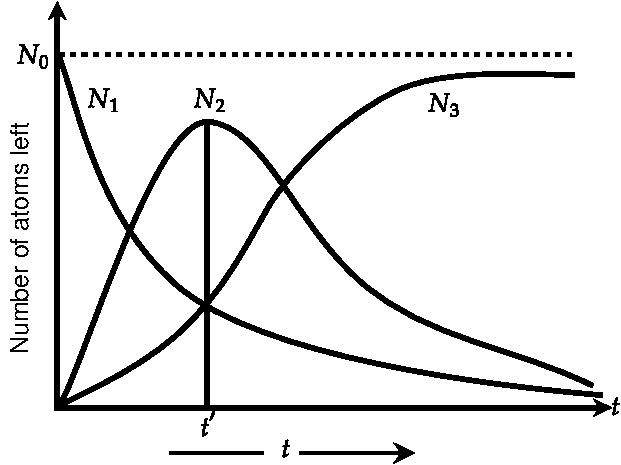
\includegraphics[height=5cm,width=7cm]{NP-8}
	\caption{}
	\label{}
\end{figure}
\textbf{(a) }When activity of the intermediate member B reaches a maximum, $t=t^{\prime}$
\begin{align*}
\left(\frac{d N_2}{d t}\right)_{t=t^{\prime}}&=0 \Rightarrow-\lambda_1 e^{-\lambda_1 t^{\prime}}+\lambda_2 e^{-\lambda_2 t^{\prime}}=0 \Rightarrow \lambda_1 e^{-\lambda_1 t^{\prime}}=\lambda_2 e^{-\lambda_2 t^{\prime}} \\
\Rightarrow t^{\prime}&=\frac{\ln \left(\lambda_2 / \lambda_1\right)}{\lambda_2-\lambda_1}
\end{align*}
\textbf{(b) Radioactive Equilibrium}\\
Any member in a radioactive chain is said to be in radioactive equilibrium with its parent when the net number of atoms of such a member does not change with time.\\
There are two type of equilibrium:
\begin{enumerate}
	\item Secular Equilibrium
$\lambda_2 \gg \lambda_1$ i.e. a long lived parent attains a state of secular equilibrium with a short lived daughter.	
	\begin{align*}
	N_2&=\frac{N_0 \lambda_1}{\lambda_2-\lambda_1}\left[e^{-\lambda_1 t}-e^{-\lambda_2 t}\right]\\
	\lambda_2-\lambda_1 &\simeq \lambda_1 \quad\text{ and after a large time has elapsed} e^{-\lambda_1 t} \gg e^{-\lambda_2 t}\\
	N_2&=\frac{N_0 \lambda_1}{\lambda_2} e^{-\lambda_1 t}=\frac{N_1 \lambda_1}{\lambda_2}, N_1 \lambda_1=N_2 \lambda_2\\
	\text{In general }&\lambda_1 N_1=\lambda_2 N_2=\lambda_3 N_3 \ldots \ldots \ldots=\lambda_n N_n\\
	\frac{N_1}{T_1}&=\frac{N_2}{T_2}=\frac{N_3}{T_3} \ldots \ldots \ldots \ldots=\frac{N_n}{T_n}
	\end{align*}
	\item Transient Equilibrium
\begin{align*}
&\text{$\lambda_2>\lambda_1$, When the parent has got a longer life time than daughter,}\\
&\text{As $e^{-\lambda_2 t}$ approaches zero; $N_2=\frac{N_0 \lambda_1}{\lambda_2-\lambda_1} e^{-\lambda_1 t} \Rightarrow N_2=\frac{N_1 \lambda_1}{\lambda_2-\lambda_1}$}\\
&\hspace{3cm} \frac{N_1}{N_2}=\frac{\lambda_2-\lambda_1}{\lambda_1}
\end{align*}
	It shows that the ratio of parent to daughter activities is a constant; such type of equilibrium is called as transient equilibrium.
	
	When the parent has got a half-life shorter than that of the daughter nucleus i.e. $\lambda_1>\lambda_2$, the state equilibrium is never achieved.
\end{enumerate}
\subsection{Alpha Decay}
Nuclei which contain 210 or more nucleons are so large that the short range nuclear forces that hold them together are barely able to counterbalance the mutual repulsion of their protons. Alpha decay occurs in such nuclei as a means of increasing their stability by reducing their size
$$
{ }_Z^A X \rightarrow{ }_{Z-2}^{A-4} Y+{ }_2^4 \mathrm{He}
$$
To escape from nucleus, a particle must have K.E., and only the alpha particle mass is sufficiently smaller than that of its constituent nucleons for such energy to be available $(\alpha$ particle have high B.E. as compared to proton or ${ }_2^3 \mathrm{He}$ nuclei).\\
The energy $Q$-released when various particles are emitted by a heavy nucleus is,\\
i.e.\\
Disintegration energy $Q=\left(m_i-m_f-m_x\right) c^2$ where \\
$m_i=$ Mass of initial nuclei,\\
$m_f=$ mass of final nuclei,\\
$m_x=\alpha$-particle mass\\
The $K E_\alpha$ of the emitted $\alpha$-particle is never quite equal to $Q$, since momentum must be conserved, the nucleus recoils with a small amount of kinetic energy when the $\alpha$-particle emerges. Thus
$$
K E_\alpha \approx\left(\frac{A-4}{A}\right) Q
$$
since $A \geq 210$, most of the disintegration energy appears as the K.E. of the $\alpha$-particle.\\\\
\textbf{Tunnel Theory of $\alpha$-decay}(How $\alpha$ particle can actually escape the nucleus)\\\\
The height of the potential barrier is $\approx 25 \mathrm{MeV}$, which is equal to the work that must be done against the repulsive electric force to bring an $\alpha$-particle from infinity to a position adjacent to the nucleus but just outside the range of its attractive forces.\\
We may therefore regard an $\alpha$-particle in such a nucleus as being inside a box whose box requires energy of $25 \mathrm{MeV}$ to be surmounted. However, decay $\alpha$-particles have energies that range from 4 to $9 \mathrm{MeV}$, depending on the particular nuclide involved, 16 to 21 $\mathrm{MeV}$ short of the energy needed for escape.
\begin{figure}[H]
	\centering
	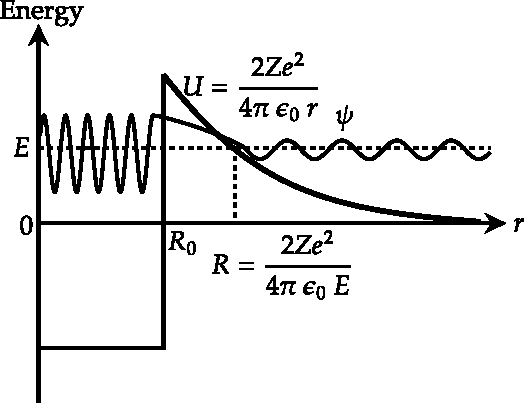
\includegraphics[height=5cm,width=6.5cm]{NP-9}
	\caption{}
	\label{}
\end{figure}
Although $\alpha$-decay is inexplicable classically,
quantum mechanics provides a straight forward explanation. The basic notions of this theory are:\\
An $\alpha$-particle may exist as an entity within a heavy nucleus. Such a particle is in constant motion and is held in the nucleus by potential barrier. There is a small but definite-likelihood that the particle may tunnel through the barrier (despite its height) each time a collision with it occurs.
\begin{align*}
&\text{The decay probability per unit time, i.e decay constant $\lambda=v T$}
\intertext{Where $v=$ number of times per second an $\alpha$-particle within a nucleus strikes the potential barrier around it and}
&\text{$T=e^{-2 k_2 L}=$ Probability that the particle will be transmitted through the barrier.}
\intertext{$L$ is the width of the barrier, wave number inside the barrier $k_2=\frac{\sqrt{2 m(U-E)}}{\hbar}$, where $E$ is the K.E., $U$ is height of the barrier and $m$ is the mass of $\alpha$-particle.}
\end{align*}
\subsection{Beta Decay}
It is a means whereby a nucleus can alter its composition to become more stable. The conservation principles of energy, linear momentum and angular momentum are all apparently violated in beta decay: $\quad n \rightarrow p+e^{-}$\\
\begin{enumerate}[label=\roman*)]
	\item  The electron energies observed in the $\beta^{-}$- decay of a particular nuclide are found to vary continuously from 0 to maximum value $K E_{\max }$ characteristic of the nuclide. The maximum energy $E_{\max }=\left(m_0 c^2+K E_{\max }\right)$ carried by the decay electron is equal to the energy equivalent of the mass difference between the parent and daughter nuclei. However an emitted electron is rarely found with energy of $K E_{\max }$.
	\begin{figure}[H]
		\centering
		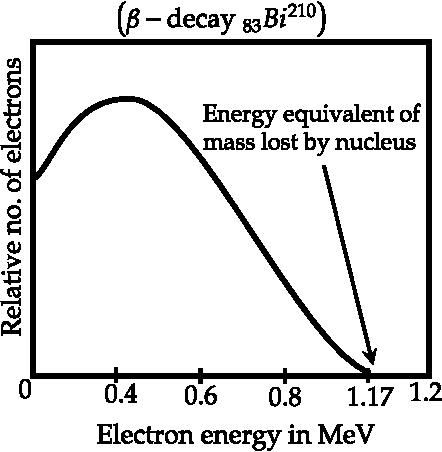
\includegraphics[height=6cm,width=6cm]{NP-10}
		\caption{}
		\label{}
	\end{figure}
\item  When the directions of emitted electron and of the recoiling nuclei are observed, they are almost never exactly opposite as required for linear momentum to be conserved.
\item (iii) The spins of the neutron, proton and electron are all $1 / 2$. If beta decay involved just a neutron becoming a proton and an electron, spin (and hence angular momentum) is not conserved.\\
In 1930 Pauli proposed a "desperate remedy": If an uncharged particle of small or zero rest mass and spin $1 / 2$ is emitted in $\beta^{-}$-decay together with the electron, the above discrepancies would not occur. This particle is called neutrino which would carry off energy equal to the difference between $K E_{\max }$ and actual $K . E$ of the electron (the recoiling nucleus carry away negligible $K . E$ ). The neutrino's linear momentum also exactly balances those of the electron and the recoiling daughter nucleus.\\
Thus in ordinary $\beta^{-}$-decay $n \rightarrow p+e^{-}+\bar{v}$ (also possible outside the nucleus)\\
The interaction of neutrinos with matter is extremely feeble. The only interaction with matter a neutrino can experience is through a process called inverse beta decay with extremely low probability $p+\bar{v} \rightarrow n+e^{+}$and $n+v \rightarrow p+e^{-}$.
\end{enumerate}
\begin{note}
	Parity violates in $\beta^{-}$- decay.
\end{note}
\subsubsection{Positron Emission}
It is the conversion of a nuclear proton into a neutron, a positron and a neutrino:
$$
p \rightarrow n+e^{+}+v \quad \text { (Possible only within a nucleus) }
$$
\subsubsection{Electron Capture}
It is closely connected with positron emission. In electron capture a nucleus absorbs one of its inner atomic electron, with the result that a nuclear proton becomes a neutron and neutrino is emitted:
$$
p+e^{-} \rightarrow n+v .
$$
Usually the absorbed electron comes from the $K$-shell, and an $X$-ray photon is emitted when one of the atoms outer electrons falls into the resulting vacant state. The wavelength of the photon will be one of those characteristic of daughter element, not of the original one, and the process can be recognized on that basis.
\begin{note}
	\begin{enumerate}
		\item Electron capture is competitive with positron emission since both processes lead to the same nuclear transformation.
		\item Electron capture occurs more often than positron emission in heavy nuclides because the electrons in such nuclides are relatively close to the nucleus, which promotes their interaction with it.
	\end{enumerate}
\end{note}
\subsubsection{Gamma Decay}
Nuclei can exist in definite energy levels just as an atom can. Due to $\alpha$ or $\beta$-emission, nuclei get into an excited state. These excited nuclei return to their ground state by emitting photons whose energies correspond to energy difference between the various initial and final states in the transition involved called $\gamma$-ray.
\begin{figure}[H]
	\centering
	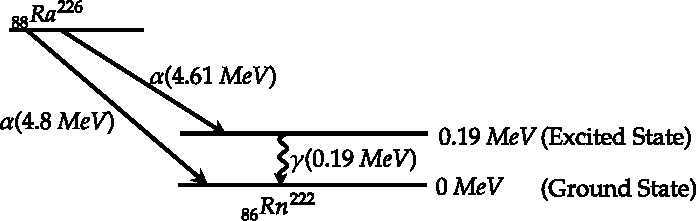
\includegraphics[height=3cm,width=9cm]{NP-11}
	\caption{}
	\label{}
\end{figure}
\subsubsection{$\gamma$-rays characteristics}
\begin{enumerate}
	\item It is an electromagnetic wave.
	\item Very short wavelength $\left(\approx 400 \mathrm{~A}^{\circ}\right.$ to $\left.0.4 \mathrm{~A}^{\circ}\right)$.
	\item No electric charge and so not detected by magnetic and electric field.
	When a beam of $\gamma$-rays photons passes through matter, the intensity of beam decreases exponentially i.e. $I=I_0 e^{-\mu x}$ where $I_0$ : Initial Intensity, $\mu$ : absorption coefficient of substance, $x$ : thickness of absorber.
\end{enumerate}
\subsubsection{Internal Conversion}
"Process of Internal Conversion is an alternative to $\gamma$-decay". Internal conversion is a process which enables an excited nuclear state to come down to some lower state without the emission of $\gamma$-photon. The energy $\Delta E$ involved in this nuclear transition gets transferred directly to a bound electron of the atom. Such an electron gets knocked out of the atom. Electrons like this are called "internal conversion" electrons.\\
This probability is highest for the $K$-shell electrons which are closest to the nucleus. For such a case, the nucleus may not de-excite by $\gamma$-emission but by giving the excitation energy $\Delta E$ directly to a $K$-shell electron. Internal conversion is also possible (though less, as compared to $K$ shell) for higher atomic shells $L, M$ etc.\\
The kinetic energy of the converted electron is $K_e=\Delta E-B_e$,\\
where $\Delta E=E_i-E_f=$ Nuclear excitation energy between initial state $i$ (higher) and final state $f$ (lower) and $B_e=$ atomic binding energy of electron.\\
We know that the $\beta$-spectrum is continuous; usually this continuous $\beta$ - spectra are superimposed by discrete lines due to conversion electrons. These lines are called 'internal conversion' lines.\\
$\gamma$-ray emission and internal conversion are competing process for de-excitation of nucleus.\\
If we neglect the small recoil energy of the $\gamma$-emitter nucleus, the energy of the $\gamma$-ray is given by $h v=\Delta E=E_i-E_f ;$ where $v$ is the frequency of the $\gamma$-photon.
\subsubsection{Pair Production (Energy into matter)}
In a collision a photon can give an electron all of its energy (the photoelectric effect) or only part (the Compton Effect). It is also possible for a photon to materialize into an electron and a positron. In this process, electromagnetic energy is converted into matter. This process is called pair production.\\
No conservation principles are violated when an electron-positron pair is created near an atomic nucleus.\\
The rest energy $m_0 c^2$ of an electron or positron is $0.51 \mathrm{MeV}$, hence pair production requires photon energy of at least $1.02 \mathrm{MeV}$. Any additional photon energy becomes $K . E$. of the electron and positron.
\begin{figure}[H]
	\centering
	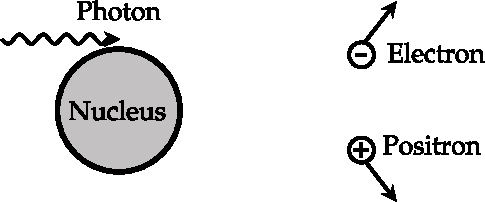
\includegraphics[height=2.5cm,width=6cm]{NP-12}
	\caption{}
	\label{}
\end{figure}
\subsubsection{Pair Annihilation}
The inverse of pair production occurs when a positron is near an electron and the two come together under the influence of their opposite electric charges. Both particles vanish simultaneously with the lost mass becoming energy in the form of two gamma ray photon.
$$
e^{+}+e^{-} \rightarrow \gamma+\gamma
$$
The total mass of the positron and electron is equivalent to $1.02 \mathrm{MeV}$, and each photon has energy $h v$ of $0.51 \mathrm{MeV}$ plus half the $K . E$. of the particles relative to their center of mass.
\begin{note}
	\begin{enumerate}
		\item The directions of the photons are such as to conserve both energy and linear momentum.
		\item No nucleus or other particles is needed for this pair annihilation to take place.
	\end{enumerate}
\end{note}
\newpage
\begin{abox}
	Practice Set-1
\end{abox}
\begin{enumerate}
	\item  A radioactive element $X$ decays to $Y$, which in turn decays to a stable element $Z$. The decay constant from $X$ to $Y$ is $\lambda_1$, and that from $Y$ to $Z$ is $\lambda_2$. If, to begin with, there are only $N_0$ atoms of $X$, at short times $\left(t \ll \frac{1}{\lambda_1}\right.$ as well as $\left.\frac{1}{\lambda_2}\right)$ the number of atoms of $Z$ will be
	{\exyear{ 	NET/JRF (JUNE-2016)}}
	 \begin{tasks}(2)
		\task[\textbf{a.}]$\frac{1}{2} \lambda_1 \lambda_2 N_0 t^2$
		\task[\textbf{b.}]$\frac{\lambda_1 \lambda_2}{2\left(\lambda_1+\lambda_2\right)} N_0 t$
		\task[\textbf{c.}]$\left(\lambda_1+\lambda_2\right)^2 N_0 t^2$
		\task[\textbf{d.}]$\left(\lambda_1+\lambda_2\right) N_0 t$
	\end{tasks}
	\item What should be the minimum energy of a photon for it to split an $\alpha$-particle at rest into a tritium and a proton?
	(The masses of ${ }_2^4 \mathrm{He},{ }_1^3 \mathrm{H}$ and ${ }_1^1 \mathrm{H}$ are $4.0026 \mathrm{amu}, 3.0161 \mathrm{amu}$ and $1.0073 \mathrm{amu}$ respectively, and $1 \mathrm{amu} \approx 938 \mathrm{MeV}$ )
	{\exyear{ NET/JRF (DEC-2016)}}
	 \begin{tasks}(4)
		\task[\textbf{a.}]$32.2 \mathrm{MeV}$
		\task[\textbf{b.}]$3 \mathrm{MeV}$
		\task[\textbf{c.}]$19.3 \mathrm{MeV}$
		\task[\textbf{d.}] $931.5 \mathrm{MeV}$
	\end{tasks}
	\item If in a spontaneous $\alpha$-decay of ${ }_{92}^{232} U$ at rest, the total energy released in the reaction is $Q$, then the energy carried by the $\alpha$-particle is
	{\exyear{ NET/JRF (JUNE-2017)}}
	 \begin{tasks}(4)
		\task[\textbf{a.}]$57 Q / 58$
		\task[\textbf{b.}]$Q / 57$
		\task[\textbf{c.}]$Q / 58$
		\task[\textbf{d.}] $23 Q / 58$
	\end{tasks}
	\item The reaction ${ }^{63} \mathrm{Cu}_{29}+p \rightarrow{ }^{63} \mathrm{Zn}_{30}+n$ is followed by a prompt $\beta$-decay of zinc ${ }^{63} \mathrm{Zn}_{30} \rightarrow{ }^{63} \mathrm{Cu}_{29}+e^{+}+v_e$. If the maximum energy of the position is $2.4 \mathrm{MeV}$, the $Q$ value of the original reaction in $\mathrm{MeV}$ is nearest to
	[Take the masses of electron, proton and neutron to be $0.5 \mathrm{MeV} / \mathrm{c}^2, 938 \mathrm{MeV} / \mathrm{c}^2$ and $939.5 \mathrm{MeV} / \mathrm{c}^2$,respectively.]
	{\exyear{ 	NET/JRF (JUNE-2018)}}
	 \begin{tasks}(4)
		\task[\textbf{a.}]$-4.4$
		\task[\textbf{b.}]$-2.4$
		\task[\textbf{c.}]$-4.8$
		\task[\textbf{d.}]$-3.4$
	\end{tasks}
\item A nucleus decays by the emission of a gamma ray from an excited state of spin parity $2^{+}$ to the ground state with spin-parity $0^{+}$what is the type of the corresponding radiation?
{\exyear{ NET/JRF (DEC-2018)}}
 \begin{tasks}(2)
	\task[\textbf{a.}]Magnetic dipole
	\task[\textbf{b.}]Electric quadrupole
	\task[\textbf{c.}]Electric dipole
	\task[\textbf{d.}]Magnetic quadrupole 
\end{tasks}
\item The ground state of ${ }_{12}^{207} \mathrm{~Pb}$ nucleus has spin-parity $J^p=\frac{1^{-}}{2}$, while the first excited state has $J^p=\frac{5^{-}}{2}$. The electromagnetic radiation emitted when the nucleus makes a transition from the first excited state to ground state are
{\exyear{ NET/JRF (JUNE-2012)}}
 \begin{tasks}(4)
	\task[\textbf{a.}]E2 and E3
	\task[\textbf{b.}]M2 or E3
	\task[\textbf{c.}]E2 or M3
	\task[\textbf{d.}]M2 or M3 
\end{tasks}
\end{enumerate}
 \colorlet{ocre1}{ocre!70!}
\colorlet{ocrel}{ocre!30!}
\setlength\arrayrulewidth{1pt}
\begin{table}[H]
	\centering
	\arrayrulecolor{ocre}
	\begin{tabular}{|p{1.5cm}|p{1.5cm}||p{1.5cm}|p{1.5cm}|}
		\hline
		\multicolumn{4}{|c|}{\textbf{Answer key}}\\\hline\hline
		\rowcolor{ocrel}Q.No.&Answer&Q.No.&Answer\\\hline
		1&\textbf{a} &2&\textbf{c}\\\hline 
		3&\textbf{a} &4&\textbf{a} \\\hline
		5&\textbf{b} &6&\textbf{c} \\\hline
		7&\textbf{}&8&\textbf{}\\\hline
		9&\textbf{}&10&\textbf{}\\\hline
		11&\textbf{} &12&\textbf{}\\\hline
		13&\textbf{}&14&\textbf{}\\\hline
		15&\textbf{}& &\\\hline
		
	\end{tabular}
\end{table}


\newpage
\begin{abox}
	Practice Set-2
\end{abox}
\begin{enumerate}
	\item A radioactive element $X$ has a half-life of 30 hours. It decays via alpha, beta and gamma emissions with the branching ratio for beta decay being $0.75$. The partial half-life for beta decay in unit of hours is---------
	{\exyear{ GATE-2019}}
	\item An $\alpha$ particle is emitted by a ${ }_{90}^{230} \mathrm{Th}$ nucleus. Assuming the potential to be purely Coulombic beyond the point of separation, the height of the Coulomb barrier is
	$\mathrm{MeV}$ ( up to two decimal places). $\quad\left(\frac{e^2}{4 \pi \epsilon_0}=1.44 \mathrm{MeV}-\mathrm{fm}, r_0=1.30 \mathrm{fm}\right.$ )
	{\exyear{ GATE-2018}}
	\item Consider the reaction ${ }_{25}^{54} \mathrm{Mn}+e^{-} \rightarrow_{24}^{54} \mathrm{Cr}+\mathrm{X}$. The particle $X$ is
	{\exyear{ 	GATE-2016}}
	 \begin{tasks}(4)
		\task[\textbf{a.}]$\gamma$
		\task[\textbf{b.}]$v_e$
		\task[\textbf{c.}]$n$
		\task[\textbf{d.}]$\pi^0$ 
	\end{tasks}
	\item In the nuclear reaction ${ }^{13} C_6+v_e \rightarrow{ }^{13} N_7+X$, the particle $X$ is
	{\exyear{ 	GATE-2017}}
	 \begin{tasks}(2)
		\task[\textbf{a.}]An electron
		\task[\textbf{b.}]An anti-electron
		\task[\textbf{c.}]A muon
		\task[\textbf{d.}]A pion 
	\end{tasks}
	\item In the $\beta$-decay of neutron $n \rightarrow p+e-\bar{v}_e$, the anti-neutrino $\bar{v}_e$, escapes detection. Its existence is inferred from the measurement of
	{\exyear{ GATE-2011}}
	 \begin{tasks}(1)
		\task[\textbf{a.}]Energy distribution of electrons
		\task[\textbf{b.}]Angular distribution of electrons
		\task[\textbf{c.}]Helicity distribution of electrons
		\task[\textbf{d.}]Forward-backward asymmetry of electrons 
	\end{tasks}
	\item In the $\beta$ decay process, the transition $2^{+} \rightarrow 3^{+}$, is
	{\exyear{ 	GATE-2013}}
	 \begin{tasks}(1)
		\task[\textbf{a.}]Allowed both by Fermi and Gamow-Teller selection rule
		\task[\textbf{b.}] Allowed by Fermi and but not by Gamow-Teller selection rule
		\task[\textbf{c.}]Not allowed by Fermi but allowed by Gamow-Teller selection rule
		\task[\textbf{d.}] Not allowed both by Fermi and Gamow-Teller selection rule
	\end{tasks}
\item  A nucleus $X$ undergoes a first forbidden $\beta$-decay to nucleus $Y$. If the angular momentum $(I)$ and parity $(P)$, denoted by $I^P$ as $\frac{7^{-}}{2}$ for $X$, which of the following is a possible $I^P$ value for $Y$ ?
{\exyear{ GATE-2014}}
	 \begin{tasks}(4)
		\task[\textbf{a.}]$\frac{1^{+}}{2}$
		\task[\textbf{b.}]$\frac{1^{-}}{2}$
		\task[\textbf{c.}]$\frac{3^{+}}{2}$
		\task[\textbf{d.}]$\frac{3^{-}}{2}$ 
	\end{tasks}
	\item A beam of $X$ - ray of intensity $I_0$ is incident normally on a metal sheet of thickness $2 \mathrm{~mm}$. The intensity of the transmitted beam is $0.025 I_0$. The linear absorption coefficient of the metal sheet $\left(\right.$ in $\left.\mathrm{m}^{-1}\right)$ is---------- (upto one decimal place)
	{\exyear{ GATE-2015}}
	\item The atomic masses of ${ }_{63}^{152} \mathrm{Eu},{ }_{62}^{152} \mathrm{Sm},{ }_1^1 \mathrm{H}$ and neutron are $151.921749,151.919756$, $1.007825$ and $1.008665$ in atomic mass units $(\mathrm{amu})$, respectively. Using the above information, the $Q$-value of the reaction ${ }_{63}^{152} E u+n \rightarrow{ }_{62}^{152} S m+p$ is ---------$\times 10^{-3}$ amu (upto three decimal places)
	{\exyear{ 	GATE-2015}}
	\item The atomic masses of ${ }_{63}^{152} \mathrm{Eu},{ }_{62}^{152} \mathrm{Sm},{ }_1^1 H$ and neutron are $151.921749,151.919756$, $1.007825$ and $1.008665$ in atomic mass units $(\mathrm{amu})$, respectively. Using the above information, the $Q$-value of the reaction ${ }_{63}^{152} E u+n \rightarrow{ }_{62}^{152} S m+p$ is ------------$\times 10^{-3}$ amu (upto three decimal places)
	{\exyear{ GATE-2015}}
\end{enumerate}
 \colorlet{ocre1}{ocre!70!}
\colorlet{ocrel}{ocre!30!}
\setlength\arrayrulewidth{1pt}
\begin{table}[H]
	\centering
	\arrayrulecolor{ocre}
	\begin{tabular}{|p{1.5cm}|p{1.5cm}||p{1.5cm}|p{1.5cm}|}
		\hline
		\multicolumn{4}{|c|}{\textbf{Answer key}}\\\hline\hline
		\rowcolor{ocrel}Q.No.&Answer&Q.No.&Answer\\\hline
		1&\textbf{40} &2&\textbf{25.995}\\\hline 
		3&\textbf{b} &4&\textbf{a} \\\hline
		5&\textbf{a} &6&\textbf{c} \\\hline
		7&\textbf{c}&8&\textbf{1844.4}\\\hline
		9&\textbf{2.833}&10&\textbf{}\\\hline
		11&\textbf{} &12&\textbf{}\\\hline
		13&\textbf{}&14&\textbf{}\\\hline
		15&\textbf{}& &\\\hline
	
	\end{tabular}
\end{table}

\newpage
\begin{abox}
	Practice Set-3
	\end{abox}
\begin{enumerate}
	\item  The half life of radioactive radon is $3.8$ day. Find the time at the end of which $(1 / 20)^{\text {th }}$ of the radon sample, will remain undecayed. (Given $\log _{10} e=0.4343$ )
	\begin{answer}
		\begin{align*}
		N&=N_0e^{-\lambda t}\text { where } \lambda=\frac{0.693}{3.8}=0.18\\
		\frac{N_0}{20}&=N_0 e^{-018 t}\text{ or }\log _{10} 20=0.18 \times t \times \log _{10} e\\
		or 1.3&=0.18 \times 0.4343 \times t\text{ or }t=\frac{1.3}{0.18 \times 0.4343} \text{or }t=16.5\text{ day}
		\end{align*}
		So the correct answer is \textbf{16.5}
	\end{answer}
		\item  A radioactive material decays by simultaneous emission of two particles with respective half-lives 1620 and 810 year. Find the time, in year, after which one-fourth of the material remains.
	\begin{answer}
		\begin{align*}
		\because \quad\frac{N}{N_0}&=e^{-\lambda t}\\
	\text{	There is a}&\text{ simultaneous emission of two particles}\\
		\therefore \quad\frac{N}{N_0}&=e^{-\left(\lambda_1+\lambda_2\right) t} \Rightarrow \frac{N_0}{4 N_0}=e^{-\left(\lambda_1+\lambda_2\right) t} \text { or } \log 4=\left(\lambda_1+\lambda_2\right) t \log e\\
		\text{Now }\lambda_1&=\frac{0.693}{1620} \lambda_2=\frac{0.693}{810}\\
		\therefore \quad2.303[2 \times 0.3]&=0.693\left[\frac{1}{1620}+\frac{1}{810}\right] t \text { or } t=\frac{2.303 \times 0.6 \times 1620}{0.693 \times 3} \text { or } t=1080 \text { year }
		\end{align*}
			So the correct answer is \textbf{1080}
	\end{answer}
		\item  A 280 day old radioactive substance shows an activity of $6000 \mathrm{dps}, 140$ day later its activity becomes 3000 dps. What was its initial activity?
	\begin{answer}
		\begin{align*}
		\text{For radioactive disintegration, }\lambda&=\frac{1}{t} \ln \frac{N_0}{N}=\frac{1}{t} \ln \left(\frac{A_0}{A}\right)\text{ or } \lambda=\frac{1}{280} \ln \left(\frac{A_0}{6000}\right)\\
		\text{also }\lambda&=\frac{1}{(280+140)} \ln \left(\frac{A_0}{3000}\right)\\
		\therefore \quad\frac{1}{280} \ln \left(\frac{A_0}{6000}\right)&=\frac{1}{420} \ln \left(\frac{A_0}{3000}\right) \text { or } 3 \ln \left(\frac{A_0}{6000}\right)=2 \ln \left(\frac{A_0}{3000}\right)\\
		\therefore\quad\left(\frac{A_0}{6000}\right)^3&=\left(\frac{A_0}{3000}\right)^2 \quad \text { or } \frac{A_0^3}{A_0^2}=\frac{(6000)^3}{(3000)^2}\\
		\text{or }A_0&=\frac{6 \times 6 \times 6 \times 10^9}{3 \times 3 \times 10^6} \quad\text{ or }A_0=24 \times 10^3 \quad\text{ or }A_0=24000\\
		\therefore\quad\text{ Initial activity }&=24000 \mathrm{dps}
		\end{align*}
			So the correct answer is \textbf{24000}
	\end{answer}
		\item Q4. A small quantity of containing $\mathrm{Na}^{24}$ radio nuclide (half life $=15$ hour) of activity $1.0$ micro curie is injected into the blood of a person $A$ sample of the blood of volume $1 \mathrm{~cm}^3$ taken after 5 hour shows an activity of 296 disintegration per minute. Determine the total volume blood in the body of the person. Assume that radioactive solution mixes uniformly in the blood of the person. ( 1 curie $=3.7 \times 10^{10}$ disintegrations per second)
	\begin{answer}
		\begin{align*}
		\text{For radioactive decay, }R&=R_0 e^{-\lambda t}\text{ or }(-\lambda t)=\ln \frac{R}{R_0}\\
		\text{or }t&=\frac{2.303}{\lambda} \log _{10}\left(\frac{R_0}{R}\right), \text{where }\lambda=\frac{0.693}{15}\text{ per hour}\\
	\text{	Half life $(T)$ }&\text{of the radio nuclide }\mathrm{Na}^{24}=15 hour\\
	\text{	Volume of blood }&=1 \mathrm{~cm}^3\text{ taken as a sample
		After 5 hour, } R=296 d p m\text{ in the blood sample.}\\
		\therefore t&=\frac{2.303}{\frac{0.693}{15}} \log _{10}\left(\frac{R_0}{296}\right) \text { or } \log _{10}\left(\frac{R_0}{296}\right)=\frac{5 \times 0.693}{2.303 \times 15} \quad \text { or } \frac{R_0}{296}=0.10033\\
		\text{or }R_0&=296 \times 1.26=373 \mathrm{dpm}\text{ or }R_0=\frac{373}{60} \mathrm{dps}\\
		\text{Activity of one micro curie }&10^{-6}\text{ curie }=3.7 \times 10^4 \mathrm{dps}\\
		\text{If activity is }&\left(\frac{373}{60}\right),\text{ volume of blood }1 \mathrm{~cm}^3\\
		\text{If activity is }&3.7 \times 10^4 \mathrm{dps}\text{ volume }=\frac{3.7 \times 10^4 \times 60}{373} \mathrm{~cm}^3\\
		\therefore\quad&\text{ Volume of blood }=5951.7 \mathrm{~cm}^3\text{ or Volume of blood }=5.95\text{ litre}\\
		\therefore \quad&\text { Total volume of blood in the body of person is } 5.95 \text { litre. }
		\end{align*}
			So the correct answer is \textbf{5.95}
	\end{answer}
		\item  A radioactive sample emits $n \beta$-particles in $2 \mathrm{sec}$ it emits $0.75 n \beta$-particles. What is the mean life of the sample? (Given $\ln 2=0.6931$ and $\ln 3=1.0986$ )
	\begin{answer}
		Let $N_0$ be the initial number of nuclei. So, after 2 seconds amount remaining $=N_0 e^{-2 \lambda}$
		\begin{align*}
		\therefore\quad &\text{ Amount dissociated, }n=N_0\left(1-e^{-2 \lambda}\right)\\
		\text{Again after 2 }&\text{ seconds amount remaining}=N_0 e^{-2 \lambda} e^{-2 \lambda}\\
		\therefore \quad &\text{Amount dissociated, }0.75 n=N_0 e^{-2 \lambda}-N_0 e^{-2 \lambda} e^{-2 \lambda}\\
		\Rightarrow 0.75&=N_0 e^{-2 \lambda}\left(1-e^{-2 \lambda}\right)\\
		\text{Solving }&\text{equations (i) and (ii)}\\
		\frac{0.75 n}{n}&=\frac{N_0 e^{-2 \lambda}\left(1-e^{-2 \lambda}\right)}{N_0\left(1-e^{-2 \lambda}\right)} \text { or, } e^{-2 \lambda}=\frac{3}{4} \Rightarrow e^{2 \lambda} \frac{4}{3} \text { or, } \ln \left(e^{2 \lambda}\right)=\ln 4-\ln 3\\
	\text{	or, }2 \lambda&=2 \ln 2-\ln 3\text{ or, }2 \lambda=2 \times 0.6931-1.0986\text{ or, }\lambda=0.1438 \sec ^{-1}\\
		\therefore\quad \text{ Mean life }&=\frac{1}{\lambda}=6.954\text{ second or mean life} =7\text{ second}
		\end{align*}
		So the correct answer is \textbf{7}
	\end{answer}
	\item  Is the $\alpha$-decay of $1^{+}$level in ${ }_{10}^{20} \mathrm{Ne}$ to $0^{+}{ }_8^{16} \mathrm{O}$ ground state possible?
	\begin{answer}
		\begin{align*}
		&\text{The decay will proceed via $l=1$ change.}\\
		&\text{From the parity selection rule, we have}\\
		&(+) \neq(+)(+)(-1)^1 \\
		&{\left[\pi_i=\pi_{\mathrm{f}} \pi_\alpha \pi_\alpha^l\right]}
	\intertext{	So the parity is not conserved. Hence, the transition is forbidden because of the nonconservation of parity.}
		\end{align*}
	\end{answer}
	\item  What is the width of the ${ }_{92}^{238} U$ coulomb barrier seen by the $\alpha$-particle. If $Q_\alpha$ of the process is $4 \cdot 27 \mathrm{MeV}$. Here coulomb barrier height $B=27 \cdot 87 \mathrm{MeV}$ ?
	\begin{answer}
		\begin{align*}
		Q_\alpha&=4 \cdot 27 \mathrm{MeV}, \quad B=27 \cdot 87 \mathrm{MeV}\\
		R&=1 \cdot 2\left(234^{1 / 3}+4^{1 / 3}\right)=9 \cdot 3 \mathrm{fm} \\
		Q_\alpha&=\frac{(Z-2) 2 e^2}{4 \pi \in_0 b}, \quad B=\frac{(Z-2) 2 e^2}{4 \pi \epsilon_0 R} \\
		\frac{Q_\alpha}{B}&=\frac{R}{b} \rightarrow b=\frac{B R}{Q_\alpha}=\frac{27 \cdot 87 \times 9 \cdot 3}{4 \cdot 27}=60 \cdot 7 \mathrm{fm}\\
		\text{The width}&\text{ of coulomb's barrier}\\
		&=b-R=60 \cdot 7-9 \cdot 3=51 \cdot 4 \mathrm{fm}
		\end{align*}
	\end{answer}
	\item  (i) Determine the number of attempts of $\alpha$ - particle per unit time trying to come out of the potential barrier for ${ }_{92}^{238} U$ nuclei. Here $Q_\alpha=4 \cdot 27 \mathrm{MeV}$,
	$$
	V_0=36 \mathrm{MeV}, m_\alpha c^2=3727 \mathrm{MeV}
	$$
	 (ii) Estimate the half life of $\alpha$-decay. If $P=2 \cdot 86 \times 10^{-39}$
	\begin{answer}
		\begin{align*}
		\text { (i):- } \frac{1}{2} m v_0^2&=Q_\alpha+V_0\\
		v_0&=\sqrt{\frac{2\left(Q_\alpha+V_0\right)}{m}}=\sqrt{\frac{2\left(Q_\alpha+V_0\right)}{m c^2}} c \\
		v_0&=\sqrt{\frac{2(4 \cdot 27+36) \mathrm{MeV}}{3727 \mathrm{MeV}}} \times 3 \times 10^8 \mathrm{~m} / \mathrm{s} \\
		&=4 \cdot 41 \times 10^7 \mathrm{~m} / \mathrm{s} \\
		f&=\frac{v_0}{2 R}=\frac{4 \cdot 41 \times 10^7}{2 \times 9 \cdot 3 \times 10^{-15}}=2 \cdot 37 \times 10^{21} \mathrm{~s}^{-1} \\
		R&=r_0\left(A_d^{1 / 3}+A_\alpha^{1 / 3}\right)=1 \cdot 2\left(234^{1 / 3}+4^{1 / 3}\right)=9.3 \mathrm{fm}\\
		\text { (ii): } T_{1 / 2}&=\frac{\ln 2}{f P}\\
		&=\frac{0 \cdot 693}{2 \cdot 37 \times 10^{21} \times 2 \cdot 86 \times 10^{-39}}\\
		&=1 \cdot 02 \times 10^{17} \mathrm{~s} \\
		&=\frac{1.02 \times 10^{17}}{365 \times 24 \times 3600} \\
		&=3 \cdot 23 \times 10^9 \mathrm{yrs}
		\end{align*}
	\end{answer}
		\item  Calculate the energy of the $\alpha$-particle emitted by ${ }_{92}^{238} U$ if $Q$. Value of the reaction is $4 \cdot 27 \mathrm{MeV}$.
		\begin{answer}
			\begin{align*}
			E_\alpha&=Q_\alpha \frac{M_d}{M_d+M_\alpha} \\
			&=4 \cdot 27 \frac{234}{234+4} \\
			E_\alpha&=4 \cdot 198 \mathrm{MeV}
			\end{align*}
		\end{answer}
	\item  What should be the pre-formation probability of the $\alpha$-cluster inside the nucleus for which the half-life of $\alpha$-decay for ${ }_{92} U^{238}$ nuclei is $4 \cdot 5 \times 10^9 y r s$. Here collision frequency $f$ and tunneling probability are $2 \cdot 37 \times 10^{21} s^{-1}$ and $2 \cdot 86 \times 10^{-39}$ respectively.
	\begin{answer}
		\begin{align*}
		\lambda&=p_\alpha f P\\
		p_\alpha&=\frac{\ln 2}{f P T_{1 / 2}}=\frac{0.693}{\left(2.37 \times 10^{21}\right)\left(2 \cdot 86 \times 10^{-39}\right)} \times 4 \cdot 5 \times 10^9 \times 365 \times 24 \times 60 \times 60 \\
		&=0.7
		\end{align*}
	\end{answer}
	\item  A nucleus with mass number 220 initially at rest emits an $\alpha$-particle. If the $Q$ value of the reaction is $5.5 \mathrm{MeV}$, calculate the kinetic energy of the $\alpha$-particle.
	\begin{answer}
		\begin{align*}
		\text{ Linear }&\text{momentum is conserved.}\\
		&X^{220} \rightarrow Y^{216}+\alpha \\
		p^y&=p^\alpha \quad p=\sqrt{2 m K} \\
		\sqrt{2(216 m) K_y}&=\sqrt{2(4 m) K_\alpha} \\
		216 K_y&=4 K_\alpha \\
		K_\alpha&=54 K_y\\
		\text{Given: }K_y+K_\alpha&=5 \cdot 5 \mathrm{MeV} \rightarrow K_y=\frac{5 \cdot 5}{55}=\frac{1}{10}=0 \cdot 1 \mathrm{MeV}\\
		K_\alpha&=54 \times 0 \cdot 1=5 \cdot 4 \mathrm{MeV}\\
	\text{	Kinetic energy}&\text{ of $\alpha$ particle }=5.4 \mathrm{MeV}\\
		\text{Binding Energy}&
		\end{align*}
	\end{answer}
	\item  If a star can convert all the He nuclei completely into oxygen nuclei, then find the energy released per oxygen nuclei. [Mass of He nucleus is $4.0026 \mathrm{amu}$ and mass of oxygen nucleus is $15.9994 \mathrm{amu}$ ].
	\begin{answer}
		\begin{align*}
		4_2 \mathrm{He}^4 \longrightarrow{ }_8 \mathrm{O}^{16}\\
	\text{	Binding energy }\Delta E&=\Delta m \times 931.5 \mathrm{MeV}\\
		&=(4 \times 4.0026-15 \cdot 9994) \times 931.5 \\
		&=10.24 \mathrm{MeV}
		\end{align*}
	\end{answer}
\end{enumerate}







